\documentclass[aspectratio=169,11pt]{beamer}

% ---------------------------------------------------------
% APRESENTACAO TP1 - COMPUTACAO GRAFICA / CCO
% Universidade Federal de Ouro Preto - DECOM
% (baseada em template_apresentacao_beamer.tex)
% ---------------------------------------------------------

% --- PACOTES PRINCIPAIS ---
\usepackage[utf8]{inputenc}
\usepackage[T1]{fontenc}
\usepackage[brazil]{babel}
\usepackage{amsmath, amssymb, amsfonts}
\usepackage{booktabs}
\usepackage{tabularx}
\usepackage{graphicx}
\usepackage{xcolor}
\usepackage{hyperref}
\usepackage{listings}
\usepackage{tikz}
\usetikzlibrary{positioning}

% --- CORES INSTITUCIONAIS / ESTILO ---
\definecolor{ufopred}{RGB}{140,29,36}
\definecolor{deepnavy}{RGB}{20,35,60}
\definecolor{lightgray}{RGB}{245,247,250}
\definecolor{darkslate}{RGB}{30,40,50}
\definecolor{softblue}{RGB}{230,238,247}

% --- TEMA BEAMER ---
\usetheme{Madrid}
\usecolortheme{default}
\setbeamertemplate{navigation symbols}{}
\setbeamercolor{structure}{fg=ufopred}
\setbeamercolor{frametitle}{fg=white,bg=ufopred}
\setbeamercolor{title}{fg=white,bg=ufopred}
\setbeamercolor{block title}{fg=white,bg=deepnavy}
\setbeamercolor{block body}{fg=black,bg=lightgray}
\setbeamercolor{alerted text}{fg=ufopred}

% --- RODAPE PERSONALIZADO ---
\setbeamertemplate{footline}{%
  \leavevmode%
  \hbox{%
    \begin{beamercolorbox}[wd=.72\paperwidth,ht=2.6ex,dp=1.1ex,leftskip=1.5ex]{author in head/foot}%
      \textcolor{darkslate}{\insertshorttitle}
    \end{beamercolorbox}%
    \begin{beamercolorbox}[wd=.28\paperwidth,ht=2.6ex,dp=1.1ex,rightskip=1.5ex plus1fil]{date in head/foot}%
      \hfill \textcolor{darkslate}{\insertframenumber/\inserttotalframenumber}
    \end{beamercolorbox}%
  }%
}

% --- CONFIGURACAO DE CODIGO ---
\lstset{
  basicstyle=\ttfamily\small,
  keywordstyle=\color{ufopred}\bfseries,
  commentstyle=\color{darkslate},
  stringstyle=\color{deepnavy},
  showstringspaces=false,
  frame=single,
  rulecolor=\color{lightgray},
  breaklines=true
}

% --- COMANDOS UTEIS ---
\newcommand{\placeholderfigure}[2][0.78\textwidth]{%
\begin{center}
\fcolorbox{deepnavy}{lightgray}{%
\begin{minipage}[c][0.30\textheight][c]{#1}
\centering
\textcolor{darkslate}{\textbf{#2}}\\[0.2cm]
\small Substitua por figura, captura de tela ou diagrama.
\end{minipage}}
\end{center}}

\newcommand{\checkitem}{\textcolor{ufopred}{$\blacktriangleright$}}

% ---------------------------------------------------------
% DADOS DA APRESENTACAO - EDITAR AQUI
% ---------------------------------------------------------
\title[Visualização CCO - Computação Gráfica]{Visualização Geométrica, Rasterização e Recorte de Árvores Arteriais CCO}
\subtitle{TP1 -- BCC327 Computação Gráfica (2026.2)}
\author{Thiago Martins Zanete \and Gabriel Barony Menezes \and Samuel Braga Marques}
\institute[UFOP]{Departamento de Computação (DECOM)\\Universidade Federal de Ouro Preto (UFOP)}
\date{BCC327 -- 2026.2}

% ---------------------------------------------------------
\begin{document}

% ---------------------------------------------------------
\begin{frame}
  \titlepage
\end{frame}

% ---------------------------------------------------------
\begin{frame}{Roteiro da Apresentação}
\tableofcontents
\end{frame}

% =========================================================
\section{Contexto e Objetivos}
% =========================================================

% ---------------------------------------------------------
\begin{frame}{Contexto do Trabalho}
\begin{block}{Problema}
Árvores arteriais geradas pelo método CCO são dados geométricos (segmentos e raios). Transformá-los em imagem envolve primitivas, transformações, rasterização e recorte, etapas que as bibliotecas gráficas costumam encapsular como uma caixa-preta.
\end{block}

\vspace{0.25cm}

\begin{itemize}
  \item Modelos CCO fornecidos pelo professor em formato \texttt{.vtk}; o método CCO \alert{não} foi reimplementado.
  \item Usamos os modelos 2D, de 8 a 256 terminais.
  \item Cada vaso é um segmento de reta com um atributo \texttt{raio}.
  \item O foco é compreender e implementar os \alert{algoritmos clássicos} de Computação Gráfica.
\end{itemize}
\end{frame}

% ---------------------------------------------------------
\begin{frame}{Objetivos}
\begin{block}{Objetivo Geral}
Desenvolver uma aplicação que integre leitura, visualização, rasterização e recorte de árvores CCO, deixando explícito o que foi implementado pelo grupo e o que veio de biblioteca.
\end{block}

\vspace{0.25cm}

\begin{itemize}
  \item Ler o modelo \texttt{VTK} e representá-lo por linhas e tubos, com cor e espessura pelo raio.
  \item Aplicar translação, rotação e escala; controlar o observador; comparar projeções.
  \item Implementar rasterização de linhas e de polígonos e comparar com e sem antialiasing.
  \item Implementar o recorte de segmentos e de polígonos.
\end{itemize}
\end{frame}

% =========================================================
\section{Dados e Metodologia}
% =========================================================

% ---------------------------------------------------------
\begin{frame}{Dados Utilizados}
\begin{columns}
\column{0.52\textwidth}
\begin{itemize}
  \item Arquivos: \texttt{tree2D\_Nterm008}, \texttt{032}, \texttt{128} e \texttt{256}\texttt{.vtk}.
  \item Formato: VTK legado ASCII, \texttt{POLYDATA}.
  \item Estrutura:
  \begin{itemize}
    \item \texttt{POINTS}: coordenadas dos pontos;
    \item \texttt{LINES}: um segmento por vaso;
    \item \texttt{CELL\_DATA}: escalar \texttt{raio}.
  \end{itemize}
  \item Com $N$ terminais: $2N$ pontos e $2N-1$ segmentos.
  \item Todos os modelos são planos ($z=0$).
\end{itemize}

\column{0.44\textwidth}
\begin{block}{Modelo analisado (8 terminais)}
\small
\begin{tabular}{ll}
\toprule
Pontos & 16\\
Segmentos & 15\\
Raio mínimo & 0,2490529\\
Raio máximo & 0,6667651\\
Dimensão & 2D\\
\bottomrule
\end{tabular}
\end{block}
\end{columns}
\end{frame}

% ---------------------------------------------------------
\begin{frame}{Tecnologias Utilizadas}
\begin{itemize}
  \item Linguagem: Python 3.10.
  \item Biblioteca gráfica: PyVista/VTK, para janela, câmera, projeções e tubos.
  \item NumPy para as matrizes; Matplotlib \alert{apenas} para exibir grades e salvar figuras.
  \item Entrada: arquivos \texttt{.vtk}. Saída: visualização interativa e figuras PNG.
\end{itemize}

\vspace{0.25cm}

\begin{block}{Ambiente de execução}
\small
Ubuntu 22.04 \quad Python 3.10 \quad PyVista 0.49.0 \quad NumPy 2.2.6\\
Intel Core i9-13900H, 16 GB \quad Intel Arc A350M\\[0.1cm]
Comando principal: \texttt{python app.py ../data/tree2D\_Nterm032.vtk}
\end{block}
\end{frame}

% ---------------------------------------------------------
\begin{frame}{Fluxo Geral da Aplicação}
\begin{columns}[T]
\column{0.50\textwidth}
\begin{center}
\begin{tikzpicture}[node distance=0.62cm, every node/.style={draw, rounded corners, align=center, minimum width=4.6cm, minimum height=0.6cm, font=\small}]
\node (vtk) {Leitura VTK};
\node (geom) [below of=vtk] {Geometria e atributos};
\node (vis) [below of=geom] {Transformações e câmera};
\node (cg) [below of=vis] {Rasterização, AA e recorte};
\node (out) [below of=cg] {Imagens e relatório};

\draw[->, thick, ufopred] (vtk) -- (geom);
\draw[->, thick, ufopred] (geom) -- (vis);
\draw[->, thick, ufopred] (vis) -- (cg);
\draw[->, thick, ufopred] (cg) -- (out);
\end{tikzpicture}
\end{center}

\column{0.47\textwidth}
\begin{block}{Código do grupo}
\small
Leitor VTK, matrizes $4\times4$, Bresenham, Scanline Fill, \emph{supersampling}, Cohen--Sutherland, Liang--Barsky e Sutherland--Hodgman.
\end{block}
\begin{block}{Biblioteca (PyVista/VTK)}
\small
Janela, câmera, vistas, projeções, tubos e mapa de cores no visualizador.
\end{block}
\end{columns}
\end{frame}

% =========================================================
\section{Implementação}
% =========================================================

% ---------------------------------------------------------
\begin{frame}{Representação Geométrica}
\small
\begin{itemize}
  \item Cada vaso é um segmento independente, com seus \alert{dois pontos próprios}: um ponto compartilhado não poderia ter três raios ao mesmo tempo.
  \item Modos (tecla \texttt{m}): linhas coloridas pelo raio; tubos (12 lados) com espessura e cor pelo raio; tubos só com espessura.
  \item Raio visual reescalado: o vaso mais grosso tem 1,5\% da maior dimensão do modelo.
\end{itemize}
\begin{center}
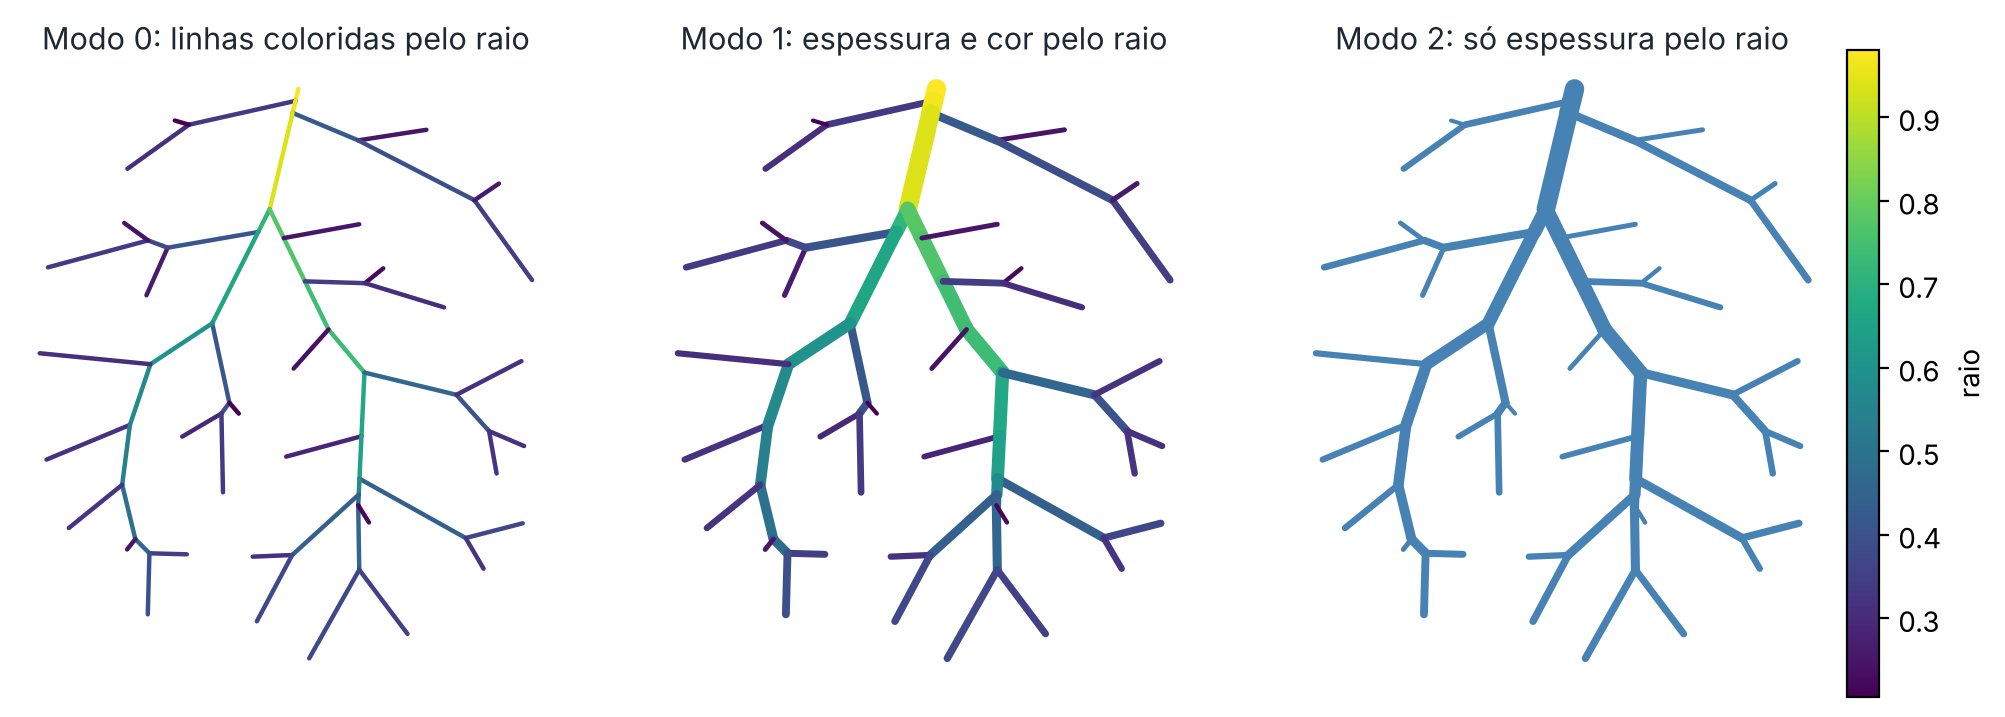
\includegraphics[height=0.42\textheight]{figures/modos_representacao.png}\\
{\scriptsize Ilustração 2D dos três modos (Matplotlib, \texttt{tree2D\_Nterm032.vtk}); o app usa tubos 3D no PyVista.}
\end{center}
\end{frame}

% ---------------------------------------------------------
\begin{frame}{Cores e Atributos Visuais}
\begin{columns}
\column{0.50\textwidth}
\begin{itemize}
  \item Mapa de cores: \emph{viridis}, contínuo, sobre $[r_{\min},r_{\max}]$ do modelo.
  \item Por que contínuo: o raio é uma grandeza escalar e ordenada.
  \item \emph{Viridis}: luminância monotônica, perceptualmente uniforme e legível com daltonismo.
  \item Barra de cores para leitura quantitativa.
  \item Espessura proporcional ao raio nos modos de tubo.
\end{itemize}

\column{0.46\textwidth}
\begin{center}
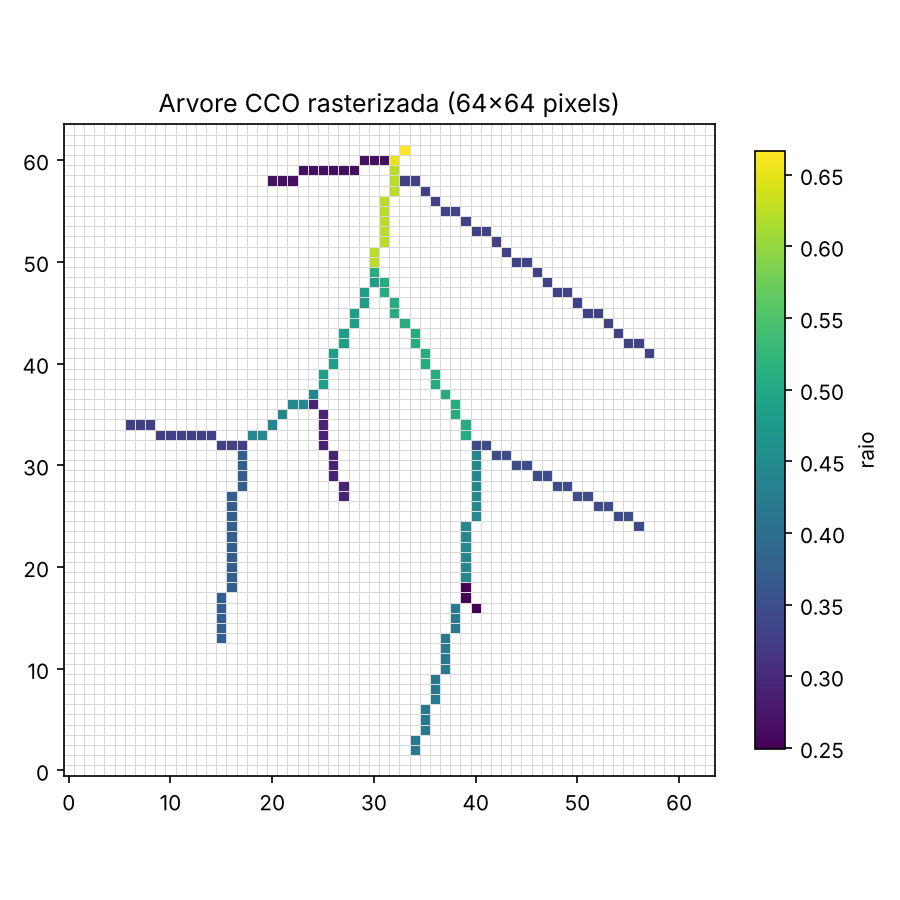
\includegraphics[height=0.62\textheight]{figures/arvore_raio.png}\\
{\scriptsize Árvore de 8 terminais: cor = raio}
\end{center}
\end{columns}
\end{frame}

% ---------------------------------------------------------
\begin{frame}{Transformações, Câmera e Projeções}
\begin{columns}[T]
\column{0.52\textwidth}
\begin{itemize}
  \item Matrizes homogêneas $4\times4$ (translação, escala, $R_x$, $R_y$, $R_z$) escritas pelo grupo.
  \item Rotação e escala em torno do centro $\mathbf{c}$ do modelo:
\end{itemize}
\[ M' = T(\mathbf{c})\,R\,T(-\mathbf{c})\,M \]
\begin{itemize}
  \item Passos: translação de 5\% do tamanho, rotação de $10^{\circ}$, escala $\times1{,}1$.
  \item Observador: vistas \texttt{xy}, \texttt{xz}, \texttt{yz}, isométrica e mouse.
\end{itemize}

\column{0.44\textwidth}
\begin{block}{Mundo $\times$ câmera}
\small
$\mathbf{p}_c = R_c^{T}(\mathbf{p}_w-\mathbf{e})$
\end{block}
\begin{block}{Projeções (tecla \texttt{o})}
\small
Ortográfica: $(x_s,y_s)=(x_c,y_c)$\\[0.1cm]
Perspectiva: $(x_s,y_s)=\left(\dfrac{f\,x_c}{z_c},\dfrac{f\,y_c}{z_c}\right)$
\end{block}
\end{columns}
\end{frame}

% ---------------------------------------------------------
\begin{frame}{Técnicas de Computação Gráfica Implementadas}
\small

\begin{tabularx}{\textwidth}{p{0.34\textwidth} X}
\toprule
\textbf{Técnica} & \textbf{Como foi utilizada no projeto}\\
\midrule
Transformações e câmera & Matrizes $4\times4$ próprias; vistas e projeções via PyVista\\
Rasterização de linhas & Bresenham (próprio), nos oito octantes\\
Rasterização de polígonos & Scanline Fill (próprio), regra par-ímpar\\
Antialiasing & \emph{Supersampling} $k\times k$ (próprio); MSAA apenas discutido\\
Recorte de segmentos & Cohen--Sutherland e Liang--Barsky (próprios); Cyrus--Beck discutido\\
Recorte de polígonos & Sutherland--Hodgman (próprio); Weiler--Atherton discutido\\
\bottomrule
\end{tabularx}

\vspace{0.2cm}
\scriptsize Visibilidade, iluminação, transparência, textura e \emph{ray casting} ficam para o TP2.
\end{frame}

% ---------------------------------------------------------
\begin{frame}{Rasterização de Linhas: Bresenham}
\begin{columns}[T]
\column{0.50\textwidth}
\small
\begin{itemize}
  \item Somente somas e comparações de \alert{inteiros}.
  \item Erro $e=\Delta x-\Delta y$ a cada passo:
  \begin{itemize}
    \item avança em $x$ se $2e>-\Delta y$;
    \item avança em $y$ se $2e<\Delta x$;
    \item as duas: passo diagonal.
  \end{itemize}
  \item Gera $\max(\Delta x,\Delta y)+1$ pixels, nos oito octantes.
  \item Exemplo $(0,0)\to(8,3)$: (0,0), (1,0), (2,1), (3,1), (4,1), (5,2), (6,2), (7,3), (8,3).
  \item Árvore de 8 terminais em $64\times64$: 173 pixels.
\end{itemize}

\column{0.48\textwidth}
\begin{center}
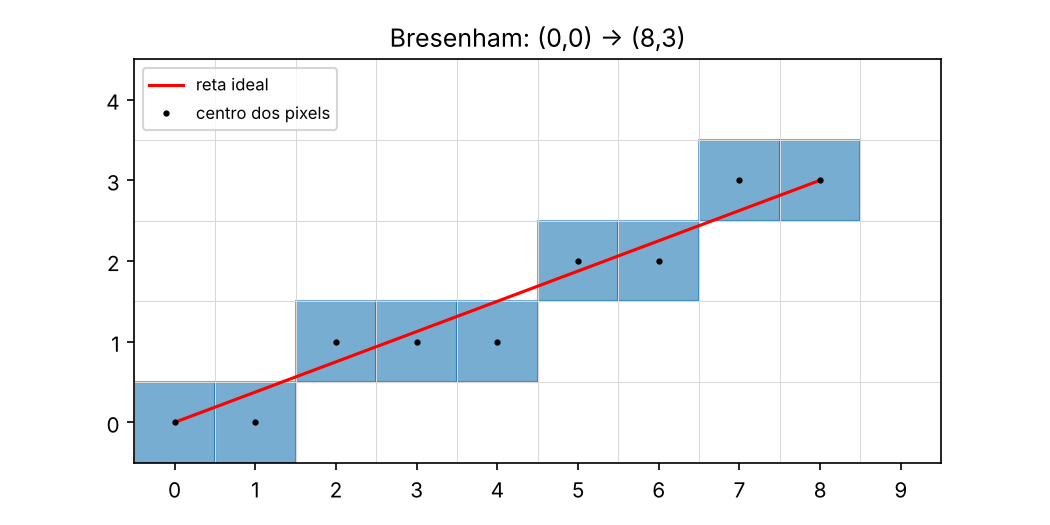
\includegraphics[width=\textwidth]{figures/bresenham_exemplo.png}\\
{\scriptsize Pixels gerados e reta ideal}
\end{center}
\end{columns}
\end{frame}

% ---------------------------------------------------------
\begin{frame}{Rasterização de Polígonos: Scanline Fill}
\begin{columns}[T]
\column{0.40\textwidth}
\small
\begin{itemize}
  \item Arestas $(y_{\min},y_{\max},x,\Delta x/\Delta y)$; horizontais ignoradas.
  \item Aresta conta se $y_{\min}\le y<y_{\max}$ (não duplica vértices).
  \item Ordena os cruzamentos e pinta pares (regra par-ímpar).
  \item U côncavo, $y=12$: cruzamentos $2{,}5;\,8{,}5;\,15{,}5;\,21{,}5$, pares $(2{,}5;8{,}5)$ e $(15{,}5;21{,}5)$.
  \item U: 222 pixels, igual à área esperada.
  \item Polígono raiz + folhas: 1695 pixels contra área exata de 1693,3.
\end{itemize}

\column{0.58\textwidth}
\begin{center}
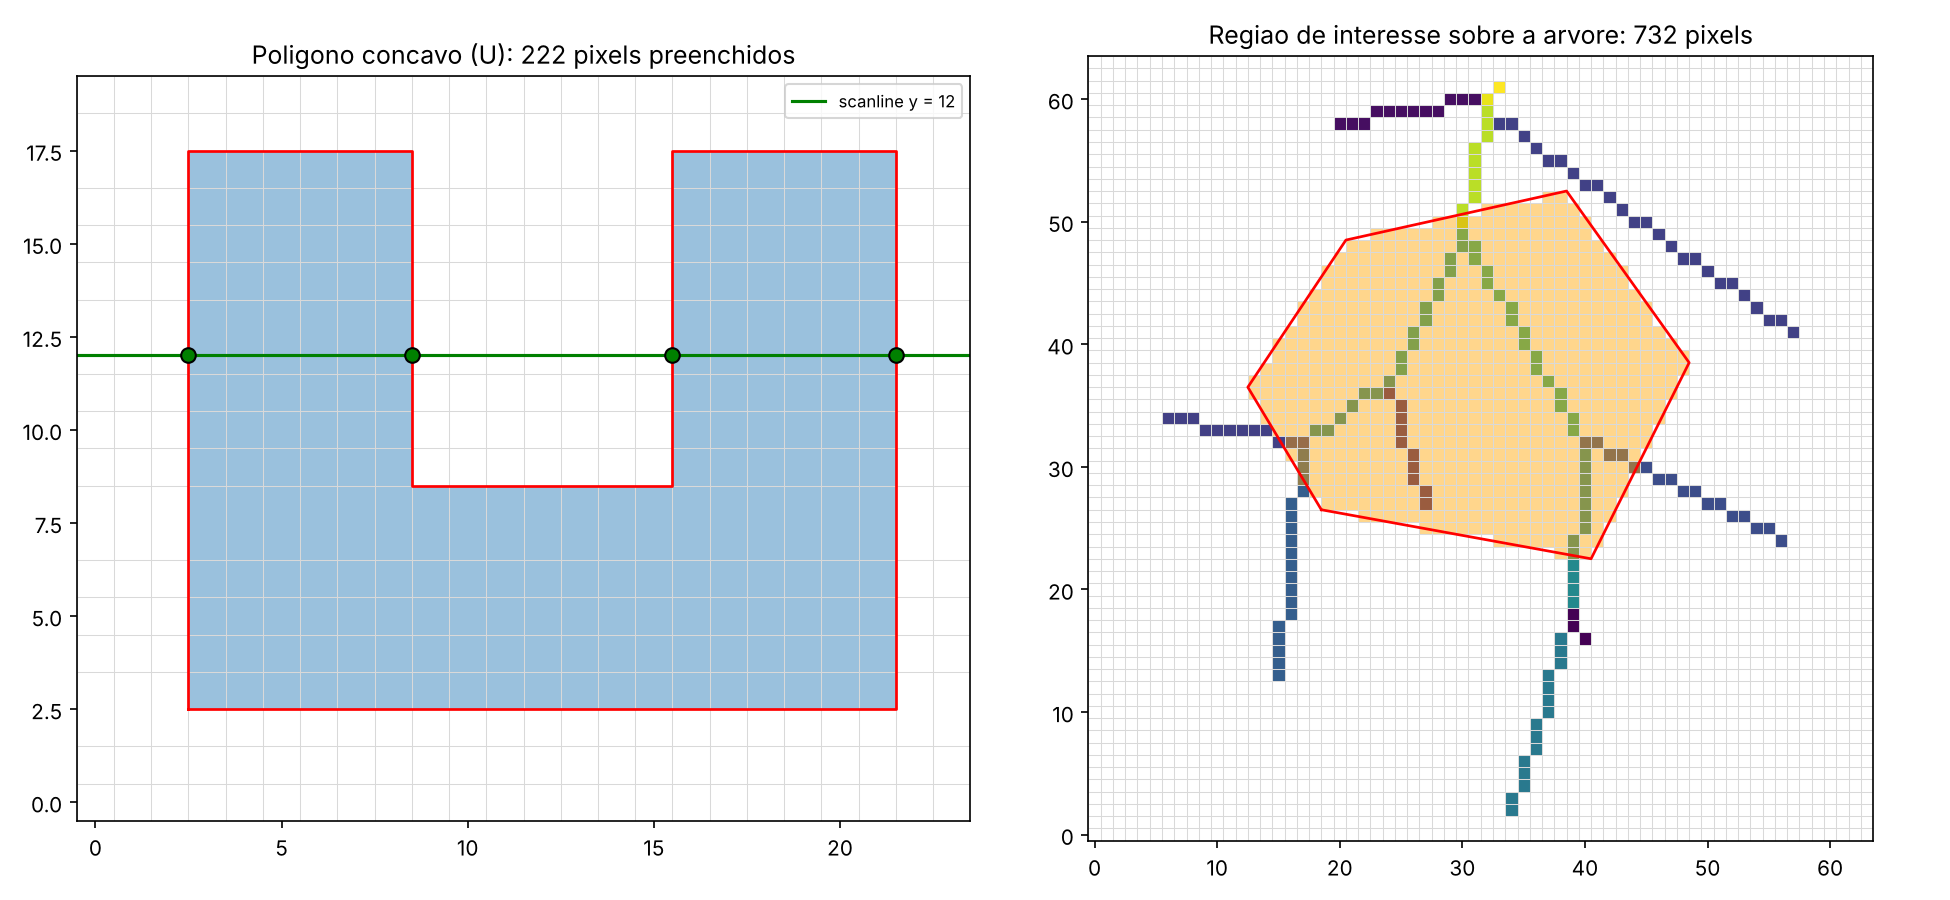
\includegraphics[width=\textwidth]{figures/scanline_fill.png}\\
{\scriptsize Polígono côncavo e região de interesse sobre a árvore}
\end{center}
\end{columns}
\end{frame}

% ---------------------------------------------------------
\begin{frame}{Aliasing e Antialiasing: Supersampling}
\begin{itemize}
  \item \alert{Aliasing}: uma amostra por pixel em linhas inclinadas e contornos produz degraus.
  \item \alert{Supersampling} com fator $k$: a cena é renderizada numa grade $k$ vezes maior em cada eixo e cada pixel recebe a \alert{média} do bloco $k\times k$ (filtro de caixa).
  \item Bordas ganham cobertura parcial, ou seja, tons intermediários.
  \item Reutiliza Bresenham (com pincel circular, para dar espessura) e Scanline Fill.
  \item MSAA (GPU): amostra a cobertura, mas calcula a cor uma vez por pixel. Só discutido.
\end{itemize}

\vspace{0.2cm}
\begin{center}
\begin{tikzpicture}[box/.style={draw, rounded corners, align=center, minimum height=0.8cm, fill=softblue, font=\small}, >=stealth]
\node[box] (a) {Cena};
\node[box, right=0.7cm of a] (b) {Grade $kn\times kn$\\ (Bresenham + Scanline)};
\node[box, right=0.7cm of b] (c) {Média de cada\\ bloco $k\times k$};
\node[box, right=0.7cm of c] (d) {Imagem\\ $n\times n$};
\draw[->, thick, ufopred] (a) -- (b);
\draw[->, thick, ufopred] (b) -- (c);
\draw[->, thick, ufopred] (c) -- (d);
\end{tikzpicture}
\end{center}
\end{frame}

% ---------------------------------------------------------
\begin{frame}{Recorte de Segmentos}
\begin{columns}[T]
\column{0.55\textwidth}
\small
\begin{itemize}
  \item \alert{Cohen--Sutherland}: código de 4 bits por extremo. Aceita se $c_0\,|\,c_1=0$; rejeita se $c_0\,\&\,c_1\neq0$; senão move um extremo até a borda e repete.
  \item \alert{Liang--Barsky}: $P(t)=P_0+t\,d$ com $p_k\,t\le q_k$ por borda. Entrada: $t_0=\max$; saída: $t_1=\min$; se $t_0>t_1$, nada é visível.
  \item \alert{Cyrus--Beck} (discutido): janela convexa qualquer, via normais. O Liang--Barsky é o caso do retângulo alinhado aos eixos.
  \item Exemplo: $(-1,7)\to(10,1)$, janela $[2,8]\times[2,6]$. Ambos chegam a $(2;5{,}364)\to(8;2{,}091)$.
\end{itemize}

\column{0.42\textwidth}
\begin{center}
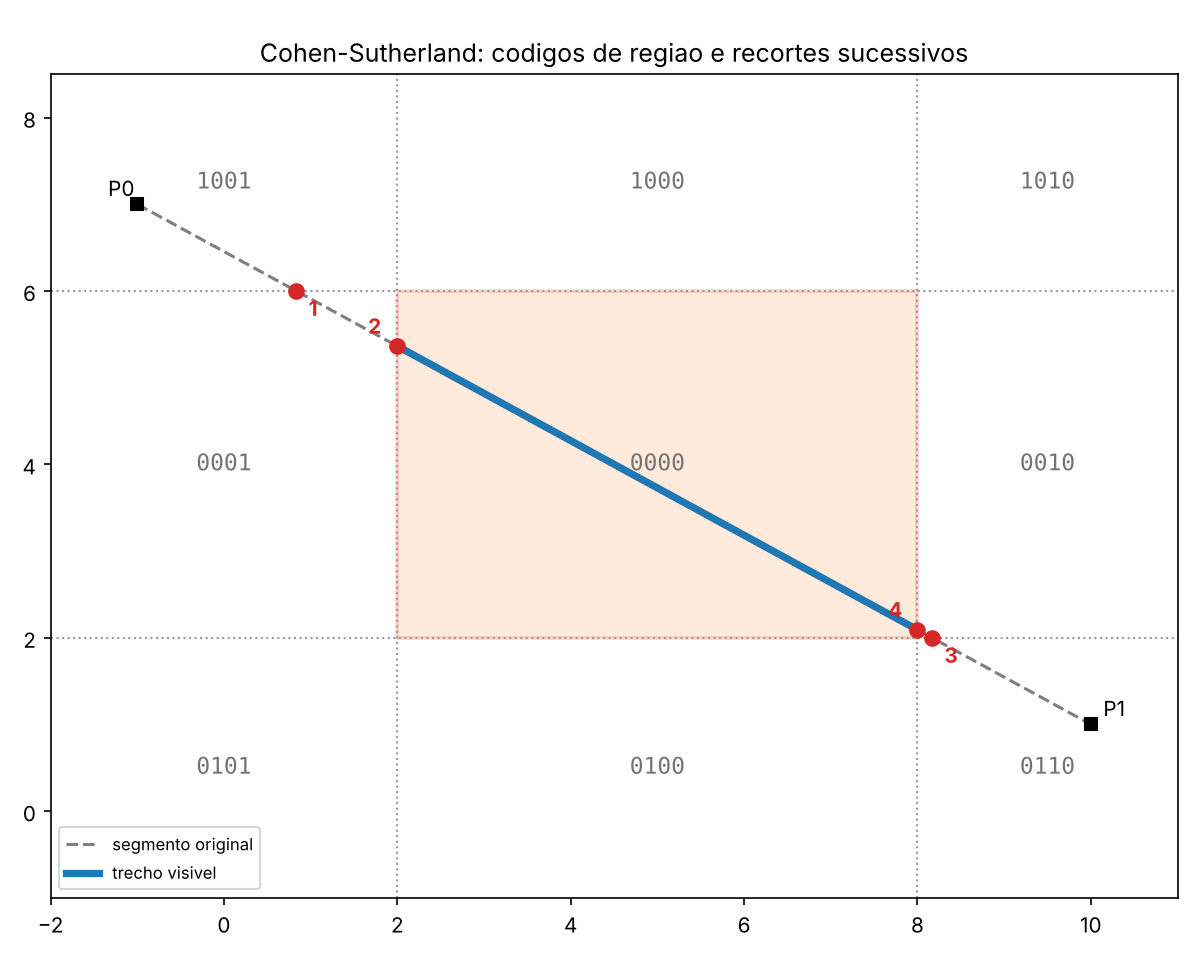
\includegraphics[width=\textwidth]{figures/recorte_exemplo.png}\\
{\scriptsize Códigos de região e recortes sucessivos}
\end{center}
\end{columns}
\end{frame}

% ---------------------------------------------------------
\begin{frame}{Recorte de Polígonos}
\begin{columns}[T]
\column{0.42\textwidth}
\small
\begin{itemize}
  \item \alert{Sutherland--Hodgman}: uma borda por vez; a saída de uma é a entrada da seguinte. Quatro regras por aresta.
  \item Exemplo (quadrilátero): $4\to5\to6\to7\to8$ vértices, área final 86,47.
  \item \alert{Limitação}: no U côncavo, o resultado são dois braços, mas a saída é \alert{uma} lista ligada por um trecho de borda percorrido nos dois sentidos. O preenchimento ainda dá os 84 pixels corretos.
  \item \alert{Weiler--Atherton} (discutido): um polígono por região; indicado para côncavos, várias regiões e furos.
\end{itemize}

\column{0.56\textwidth}
\begin{center}
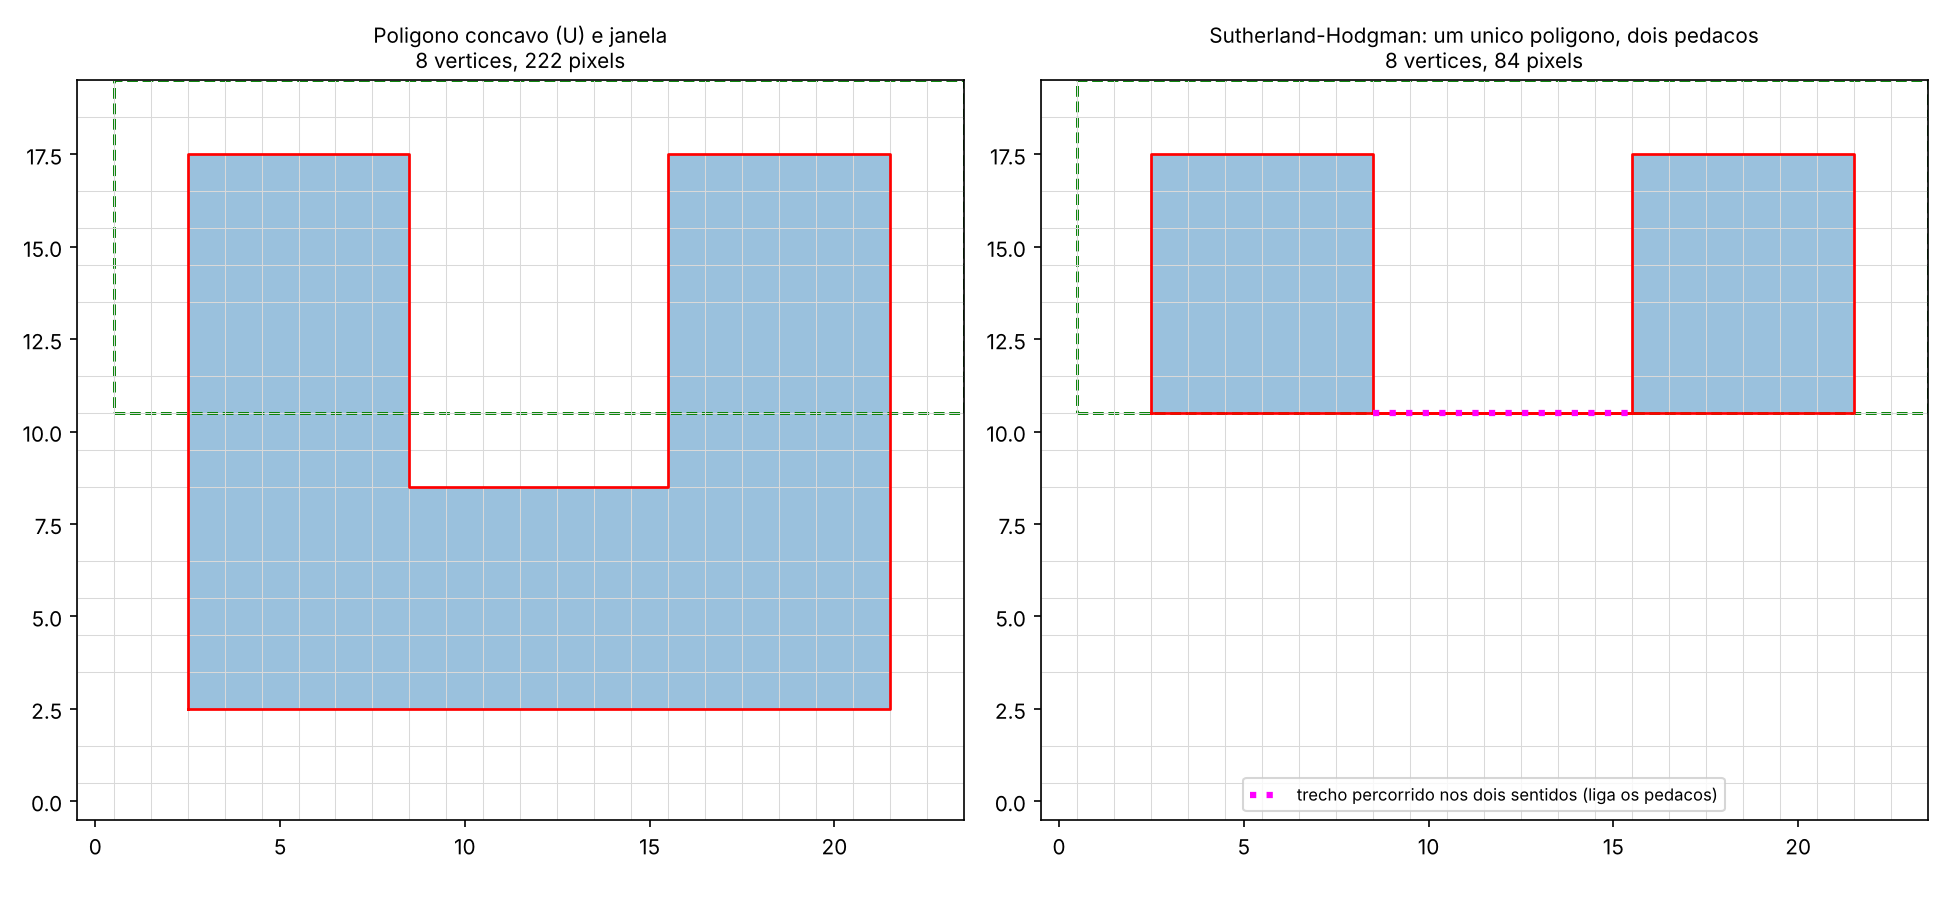
\includegraphics[width=\textwidth]{figures/recorte_poligono_concavo.png}\\
{\scriptsize U côncavo recortado por $y\ge10{,}5$}
\end{center}
\end{columns}
\end{frame}

% =========================================================
\section{Resultados}
% =========================================================

% ---------------------------------------------------------
\begin{frame}{Resultados Principais}
\begin{columns}
\column{0.49\textwidth}
\begin{center}
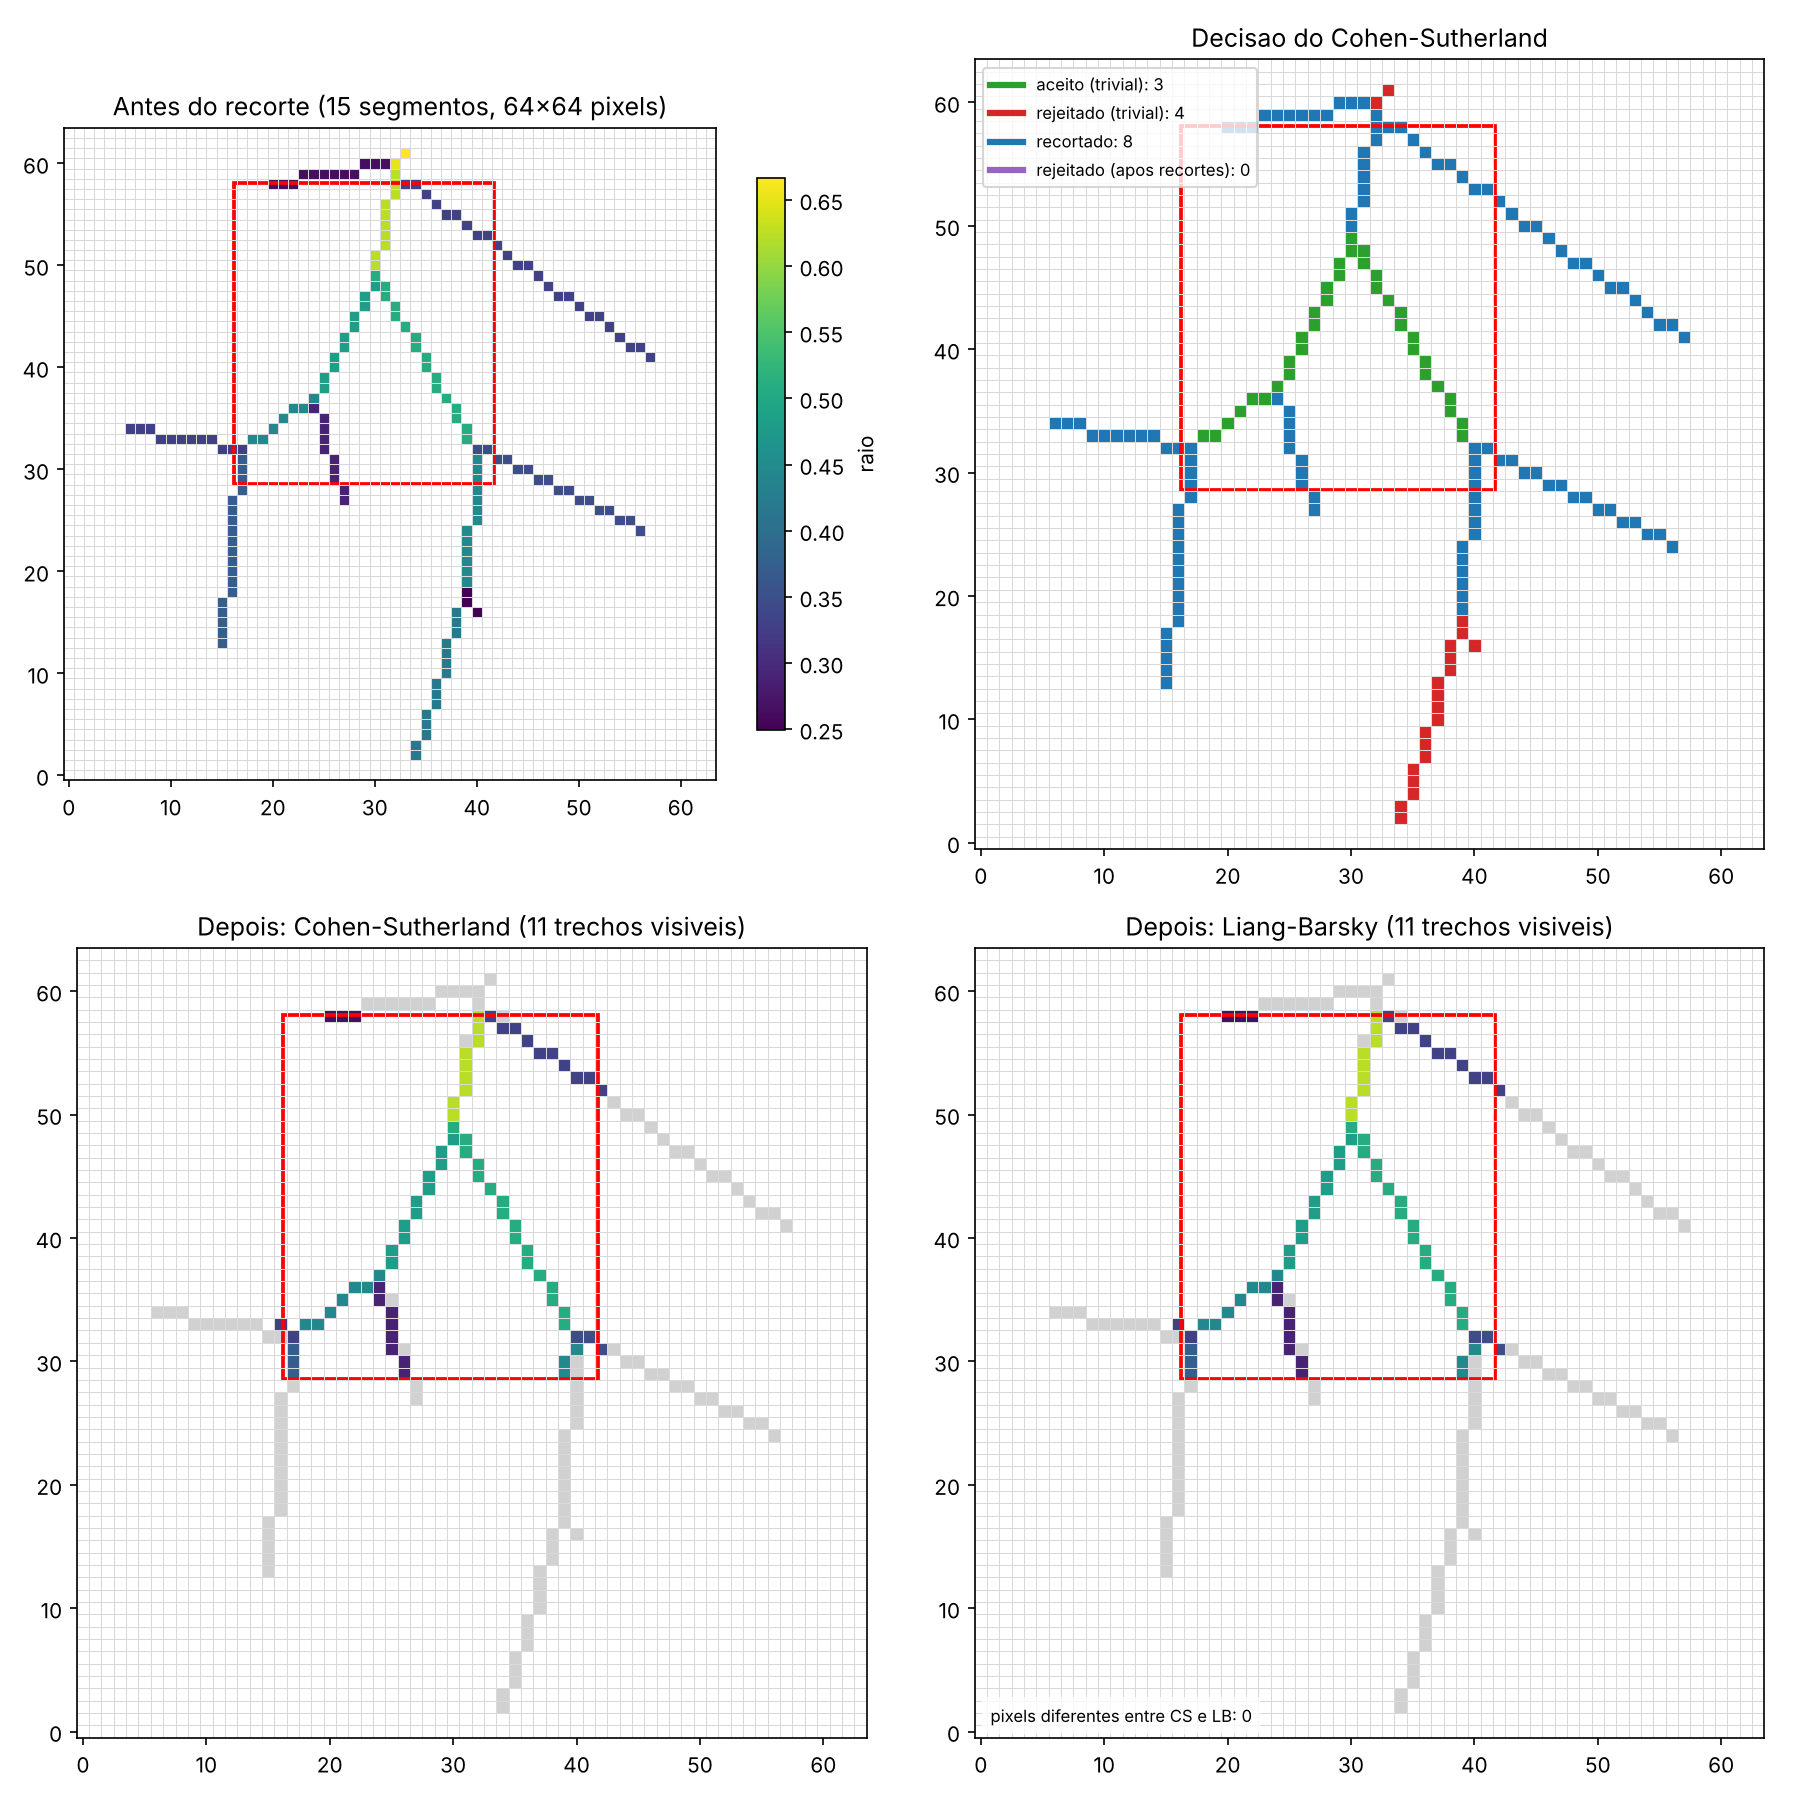
\includegraphics[height=0.66\textheight]{figures/recorte_arvore.png}
\end{center}
\column{0.49\textwidth}
\begin{center}
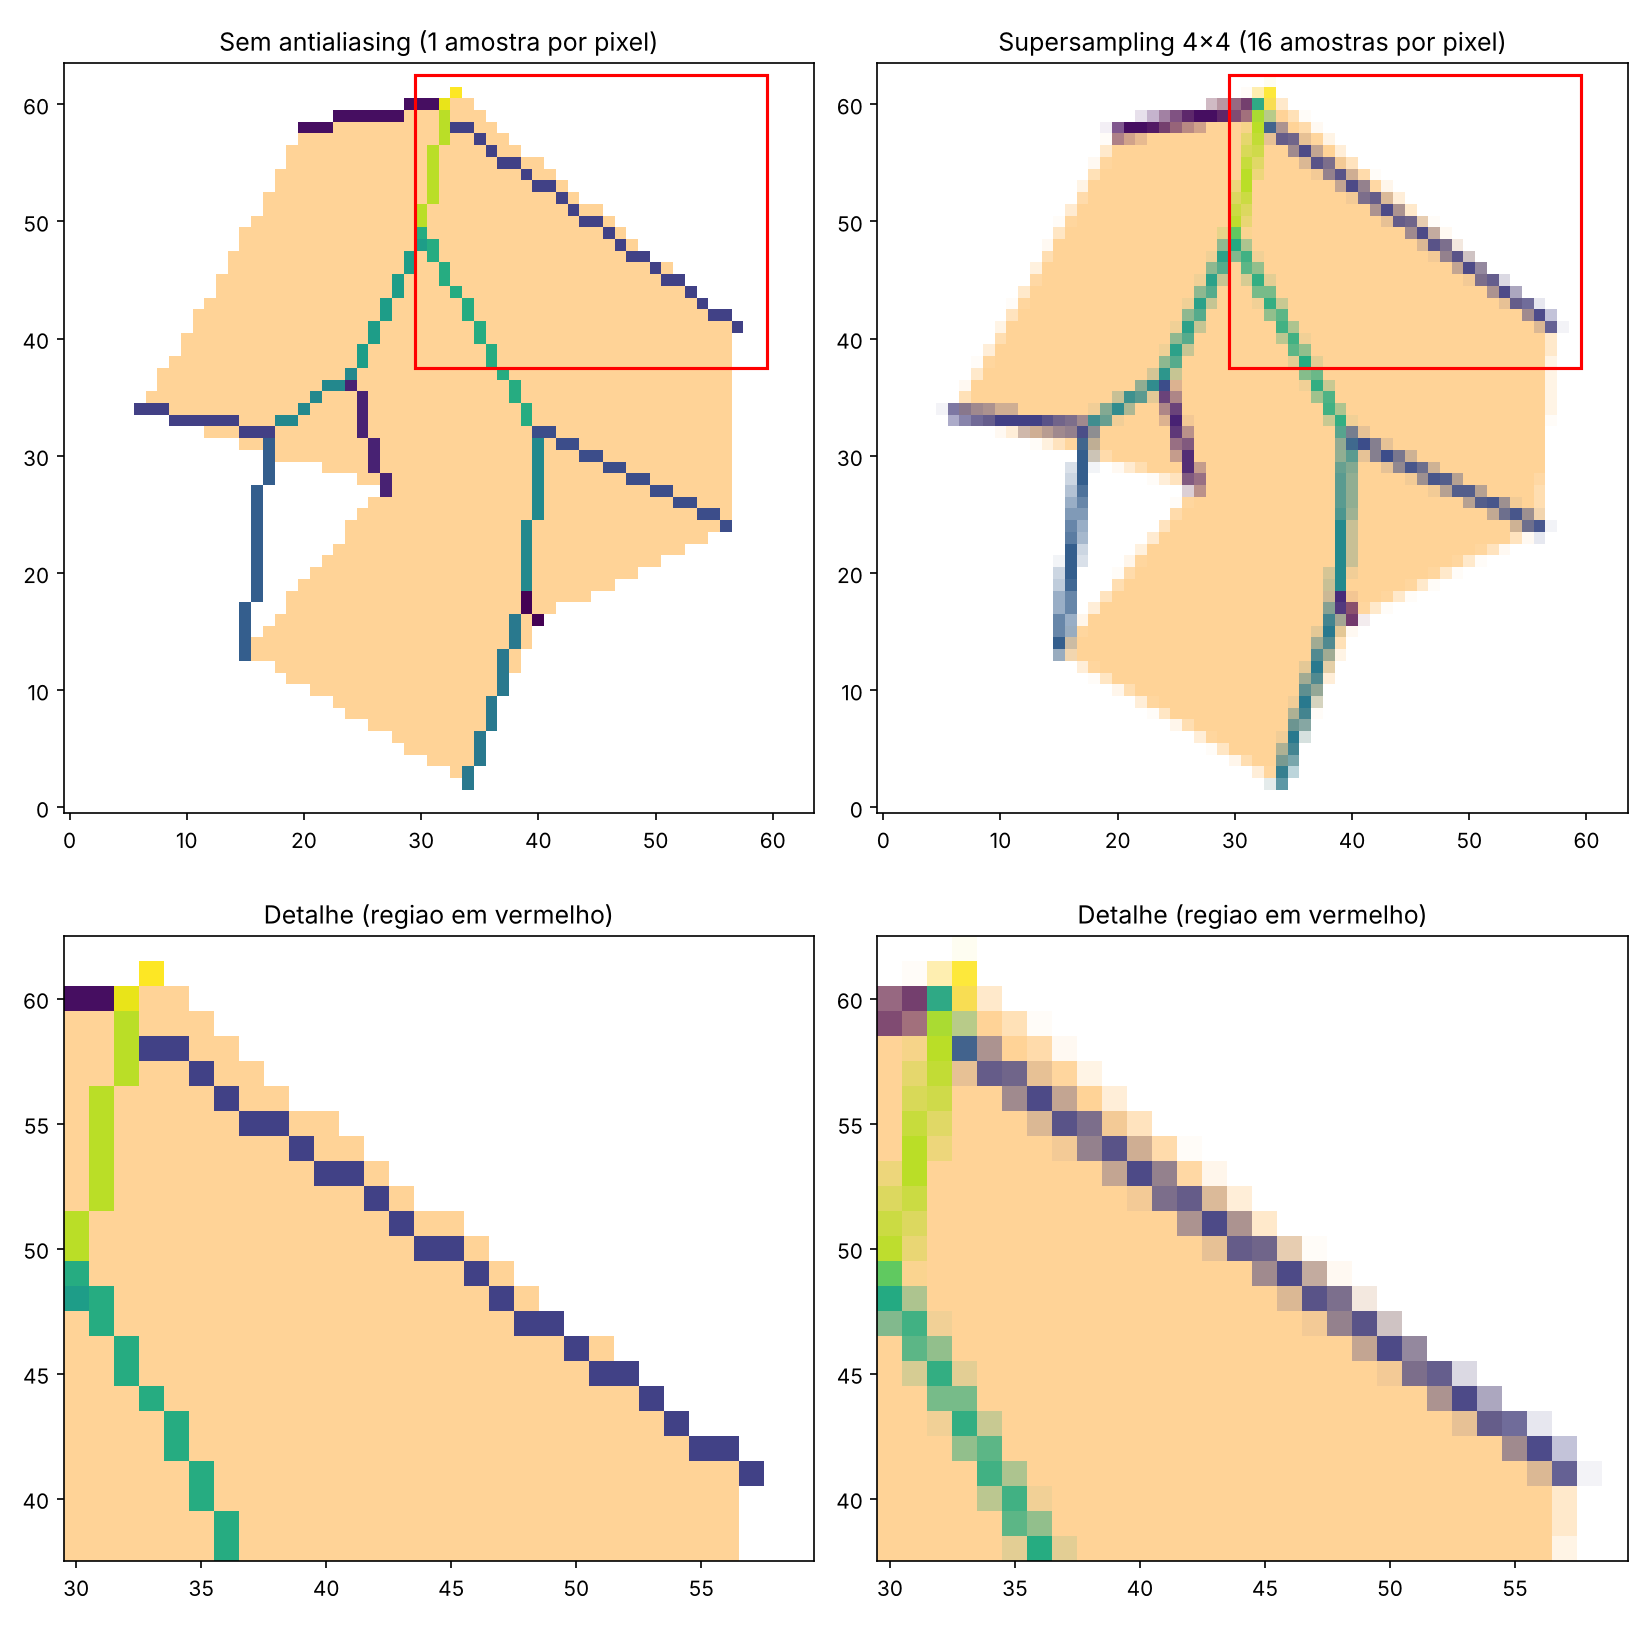
\includegraphics[height=0.66\textheight]{figures/antialiasing.png}
\end{center}
\end{columns}

\vspace{0.1cm}
\scriptsize
\textbf{Esq.:} recorte da árvore em $64\times64$ pixels. Dos 15 segmentos, 3 foram aceitos, 4 rejeitados e 8 recortados (173 $\to$ 76 pixels pintados); Cohen--Sutherland e Liang--Barsky geram a mesma imagem. \textbf{Dir.:} sem antialiasing e com \emph{supersampling} $4\times4$.
\end{frame}

% ---------------------------------------------------------
\begin{frame}{Comparações Realizadas}
\begin{columns}[T]
\column{0.47\textwidth}
\begin{block}{Sem $\times$ com antialiasing (EQM)}
\small
\begin{tabular}{lcccc}
\toprule
$k$ & 1 & 2 & 4 & 8\\
\midrule
EQM ($\times10^{-3}$) & 4,68 & 1,72 & 0,24 & 0,03\\
\bottomrule
\end{tabular}\\[0.15cm]
Referência: $16\times16$ amostras. Tons distintos: 17 (sem AA) e 200 ($k=4$). O erro cai cerca de 20 vezes entre $k=1$ e $k=4$.
\end{block}

\column{0.50\textwidth}
\begin{block}{Cohen--Sutherland $\times$ Liang--Barsky}
\small
\begin{tabular}{lcc}
\toprule
& CS & LB\\
\midrule
Estratégia & códigos de região & parâmetro $t$\\
Janela & retângulo & retângulo\\
Resultado & \multicolumn{2}{c}{idêntico}\\
\bottomrule
\end{tabular}\\[0.15cm]
Idênticos em 40\,000 segmentos aleatórios e em 0 pixels de diferença na árvore. O custo relativo depende da implementação.
\end{block}
\end{columns}

\vspace{0.1cm}
\small
\begin{itemize}
  \item Ortográfica $\times$ perspectiva: comparada no visualizador (tecla \texttt{o}) com o modelo plano inclinado.
\end{itemize}
\end{frame}

% ---------------------------------------------------------
\begin{frame}{Recurso Adicional: Recorte Interativo}
\begin{columns}
\column{0.52\textwidth}
\begin{block}{Recurso implementado}
\small
Janela de recorte sobre o modelo no visualizador (\texttt{app.py}), com troca de algoritmo em tempo real.
\end{block}
\small
\begin{itemize}
  \item \textbf{Motivação:} ver o recorte atuando sobre o modelo, não só em figuras estáticas.
  \item \textbf{Como:} janela vermelha móvel e redimensionável (\texttt{h j k l}, \texttt{,} \texttt{.}); tecla \texttt{1} liga/desliga; tecla \texttt{2} alterna Cohen--Sutherland e Liang--Barsky; $z$ interpolado ao longo do segmento.
  \item \textbf{Resultado:} árvore original em cinza, trechos visíveis coloridos pelo raio e contagem \texttt{n/N} segmentos visíveis na tela.
\end{itemize}

\column{0.44\textwidth}
\begin{center}
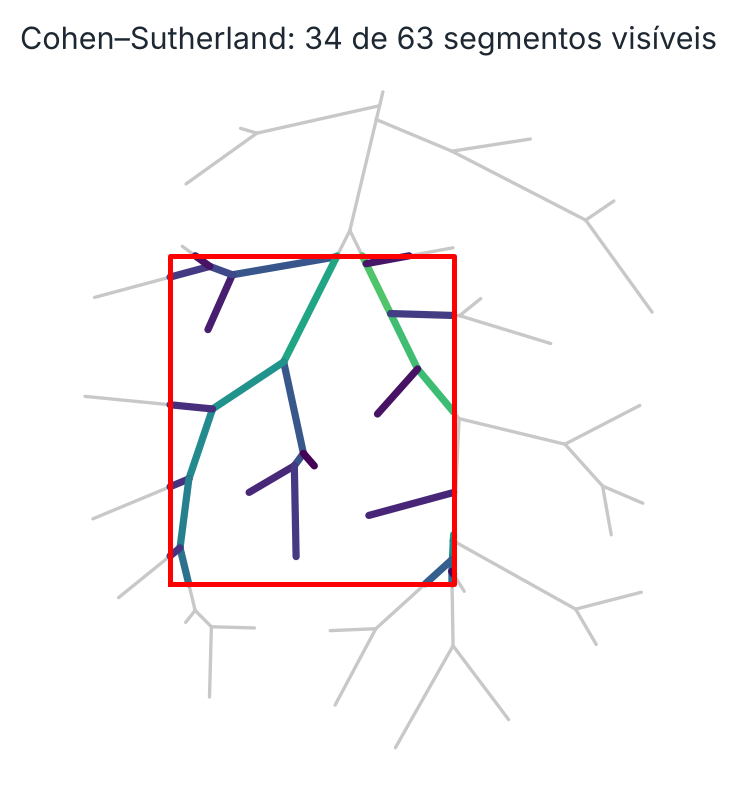
\includegraphics[height=0.52\textheight]{figures/recorte_modelo.png}\\
{\scriptsize Ilustração do resultado exibido (Matplotlib, mesmo Cohen--Sutherland), 32 terminais}\\[0.1cm]
{\scriptsize \texttt{python app.py ../data/tree2D\_Nterm032.vtk}\\ \texttt{--recorte --algoritmo 1}}
\end{center}
\end{columns}
\end{frame}

% =========================================================
\section{Discussão e Conclusão}
% =========================================================

% ---------------------------------------------------------
\begin{frame}{Discussão}
\small
\begin{itemize}
  \item \textbf{Conceitos aplicados:} coordenadas homogêneas, mundo e câmera, projeções, Bresenham, Scanline, \emph{supersampling}, Cohen--Sutherland, Liang--Barsky e Sutherland--Hodgman.
  \item \textbf{Dificuldades:} casos degenerados (vértices sobre a borda, segmentos paralelos, pontos) e convenções de pixel e de borda, resolvidos com regras explícitas e testes contra métodos independentes.
  \item \textbf{Com biblioteca:} janela, câmera, projeções, tubos e mapa de cores (PyVista/VTK).
  \item \textbf{Pelo grupo:} leitor VTK, matrizes, rasterização, antialiasing e recorte.
  \item \textbf{Limitações e melhorias:} só modelos 2D foram usados; o antialiasing não tem tecla no \texttt{app.py}; o recorte do app é feito no espaço do modelo; implementar Weiler--Atherton e testar modelos 3D.
\end{itemize}
\end{frame}

% ---------------------------------------------------------
\begin{frame}{Conclusões}
\begin{itemize}
  \item Os algoritmos de rasterização e recorte foram implementados e conferidos contra métodos independentes: 202 polígonos (Scanline), 40\,000 segmentos (recorte) e 300 polígonos (Sutherland--Hodgman).
  \item O \emph{supersampling} $4\times4$ reduziu o erro cerca de 20 vezes; Cohen--Sutherland e Liang--Barsky concordaram em todos os testes.
  \item Objetivos do TP1 cumpridos, com a divisão entre código próprio e biblioteca documentada.
  \item O raio como atributo, mapeado em cor e espessura, é o uso típico de visualização científica de dados vasculares.
\end{itemize}

\vspace{0.25cm}

\begin{block}{Mensagem final}
Implementar e verificar os algoritmos clássicos mostra o que o \emph{pipeline} gráfico faz por trás da biblioteca, e é a base para visibilidade, iluminação e textura no TP2.
\end{block}
\end{frame}

% ---------------------------------------------------------
\begin{frame}{Referências}
\footnotesize
\begin{thebibliography}{99}
\bibitem{schreiner1993} SCHREINER, W.; BUXBAUM, P. Computer-optimization of vascular trees. \textit{IEEE Transactions on Biomedical Engineering}, 1993.
\bibitem{foley} FOLEY, J. D. et al. \textit{Computer Graphics: Principles and Practice}. Addison-Wesley.
\bibitem{bresenham} BRESENHAM, J. E. Algorithm for computer control of a digital plotter. \textit{IBM Systems Journal}, 1965.
\bibitem{liang} LIANG, Y.-D.; BARSKY, B. A. A new concept and method for line clipping. \textit{ACM Transactions on Graphics}, 1984.
\bibitem{sh} SUTHERLAND, I. E.; HODGMAN, G. W. Reentrant polygon clipping. \textit{Communications of the ACM}, 1974.
\bibitem{wa} WEILER, K.; ATHERTON, P. Hidden surface removal using polygon area sorting. \textit{SIGGRAPH}, 1977.
\bibitem{pyvista} SULLIVAN, C. B.; KASZYNSKI, A. PyVista. \textit{Journal of Open Source Software}, 2019.
\bibitem{vtk} VTK Documentation. \url{https://vtk.org/}
\end{thebibliography}
\end{frame}

% ---------------------------------------------------------
\appendix
\section{Apêndice}

\begin{frame}[fragile]{Comandos de Execução}
\begin{lstlisting}[language=bash]
cd src
python app.py ../data/tree2D_Nterm032.vtk                    # visualizador
python app.py ../data/tree2D_Nterm032.vtk --recorte --algoritmo 1
python bresenham.py     ../data/tree2D_Nterm008.vtk
python scanlineFill.py  ../data/tree2D_Nterm008.vtk
python antiAliasing.py  ../data/tree2D_Nterm008.vtk
python recorteSegmentos.py ../data/tree2D_Nterm008.vtk
python recorteArvore.py    ../data/tree2D_Nterm008.vtk
python recortePoligonos.py ../data/tree2D_Nterm008.vtk
\end{lstlisting}

\begin{block}{Observação}
\small
Os módulos didáticos gravam as figuras em \texttt{../figures}.
\end{block}
\end{frame}

\begin{frame}{Comandos de Teclado e Mouse (\texttt{app.py})}
\footnotesize
\begin{tabularx}{\textwidth}{l X}
\toprule
\textbf{Entrada} & \textbf{Ação}\\
\midrule
Mouse: esquerdo / roda / meio & Girar / zoom / mover a câmera\\
\texttt{m} \texttt{v} \texttt{o} \texttt{0} & Modo de desenho; vista; ortográfica/perspectiva; restaurar o modelo\\
Setas; \texttt{+} \texttt{-} & Transladar; escala $\times1{,}1$ e $\times1/1{,}1$\\
\texttt{z} \texttt{x} / \texttt{a} \texttt{d} / \texttt{u} \texttt{i} & Rotação em $Z$ / $Y$ / $X$ ($\pm10^{\circ}$)\\
\texttt{1} \texttt{2} & Liga/desliga o recorte; troca o algoritmo\\
\texttt{h} \texttt{l} \texttt{j} \texttt{k}; \texttt{,} \texttt{.} & Move a janela de recorte; reduz/amplia a janela\\
\bottomrule
\end{tabularx}
\end{frame}

\begin{frame}{Verificação Automática}
\small
\begin{itemize}
  \item \textbf{Bresenham:} extremos, contagem $\max(\Delta x,\Delta y)+1$, pixels vizinhos e desvio $\le0{,}5$ da reta ideal.
  \item \textbf{Scanline:} comparado ao teste do raio em 202 polígonos (U, hexágono e 200 aleatórios).
  \item \textbf{Recorte de segmentos:} 11 casos fixos e 40\,000 aleatórios; CS = LB, extremos na janela e sobre a reta, trecho maximal.
  \item \textbf{Sutherland--Hodgman:} 4 casos fixos e 300 polígonos aleatórios, conferidos pixel a pixel.
\end{itemize}
\end{frame}

\begin{frame}[fragile]{Núcleo do Bresenham}
\begin{lstlisting}[language=Python]
dx, dy = abs(x1 - x0), abs(y1 - y0)
sx = 1 if x0 < x1 else -1
sy = 1 if y0 < y1 else -1
erro = dx - dy
x, y = x0, y0
while True:
    pixels.append((x, y))
    if x == x1 and y == y1:
        break
    e2 = 2 * erro              # dobro do erro evita fracoes
    if e2 > -dy:               # precisa avancar em x
        erro -= dy
        x += sx
    if e2 < dx:                # precisa avancar em y
        erro += dx
        y += sy
\end{lstlisting}
\end{frame}

\begin{frame}{Obrigado!}
\begin{center}
{\Huge Obrigado!}\\[0.5cm]
{\large Perguntas?}\\[0.5cm]
{\small \texttt{thiago.zanete@aluno.ufop.edu.br}\\ \texttt{gabriel.barony@aluno.ufop.edu.br}\\ \texttt{samuel.bm@aluno.ufop.edu.br}}
\end{center}
\end{frame}

\end{document}
